\documentclass{article}
\usepackage[left=2cm, right=2cm, top=2cm]{geometry}
%%%%%%%%%%%%%%%%%%%%%%%%%%%%%%%%%% PACKAGES %%%%%%%%%%%%%%%%%%%%%%%%%%%%%%%%%%
\usepackage{minted}                     % Code
\usepackage{graphicx}                   % PNGs
\usepackage{algorithm}
\usepackage{algpseudocode}              % Algorithms
\usepackage{amsmath}                    % Rightarrow
\usepackage{hyperref}                   % Hyperlinks
\hypersetup{
    colorlinks,
    linkcolor=black
}

%%%%%%%%%%%%%%%%%%%%%%%%%%%%%%%%%%%%%%%%%%%%%%%%%%%%%%%%%%%%%%%%%%%%%%%%%%%%%%%

\pagenumbering{gobble}

\title{\textbf{Programming Assignment #2}}
\author{MacMillan, Kyle}
\date{November 12, 2018}


\begin{document}

\maketitle
\addcontentsline{toc}{section}{Title}

\newpage
\pagenumbering{roman}   % Set TOC page numbering to lowercase roman numerals
\tableofcontents
\addcontentsline{toc}{section}{Table of Contents}

\newpage
\listoffigures
\addcontentsline{toc}{section}{List of Figures}

\listofalgorithms
\addcontentsline{toc}{section}{List of Algorithms}

\newpage
\pagenumbering{arabic}  % Set content page numbering to arabic numerals
% Setup Hyperlinks for the rest of the document
\hypersetup{
    colorlinks,
    citecolor=blue,
    filecolor=black,
    linkcolor=blue,
    urlcolor=blue
}

\section{Description of the program}
\setcounter{page}{1} % Set the page counter to 3
asdf


\section{Description of the algorithms and libraries used}
asdf


\section{Description of functions and program structure}
asdf


\section{How to compile and use the program}
asdf

\newpage
\section{Description of the testing and verification process}
To test this I began with a sanity check function to ensure I was even 
performing the matrix-vector multiplication as expected. I took a simple $3x3$ 
matrix and multiplied it with a $3x1$ vector. I verified the output was correct 
and then pressed on. After learning more about CUDA and what was going on I 
determined a $3x3$ matrix was not sufficient to test. It is too cumbersome to 
come up with a testable $N x N$ matrix of sufficient size so I used the identity 
matrix because $AI = A$ so I was able to easily perform a sanity check where $A$ 
was represented with an ascending number of integers. 

After verifying the correctness of the algorithm I tested the speed of a 
single-threaded version of the algorithm, as can be seen in Figure \ref{fig:slow}.

\begin{figure}[h]
    \centering
    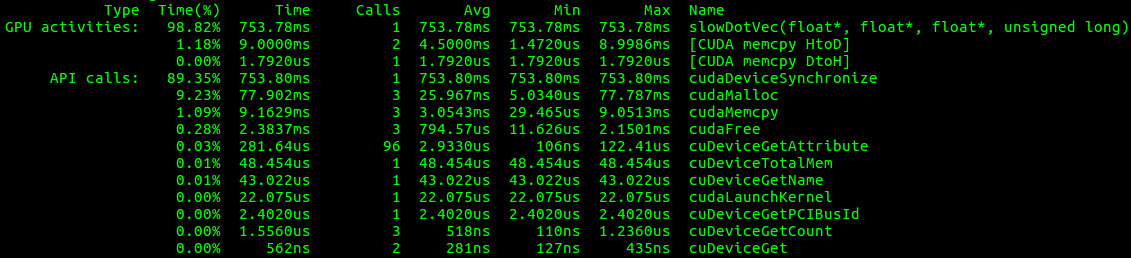
\includegraphics[width=0.95\textwidth]{slow}
    \caption{Single Thread Matrix * Vector}
    \label{fig:slow}
\end{figure}

I then compared that to the fully-parallelized version of the code, as shown in 
Figure \ref{fig:fast}. If we compare the function runtime of the single-threaded 
and multi-threaded functions we see they took $753780us$ and 
$1968.9us + 3.04us = 1971.94us$ respectively. That is a speedup of about $382.5$ 
times faster utilizing the full power of the CUDA cores. We can then calculate 
the Karp-Flatt metrix using $p=1024$ as:

$$e = \frac{\frac{1}{\psi} - \frac{1}{p}}{1 - \frac{1}{p}}$$
$$\frac{1}{\psi} = 0.002616068$$
$$\frac{1}{p} = 0.000976562$$

Which yields a Karp-Flatt metric of:
$$e = 0.001641108$$

\begin{figure}[h]
    \centering
    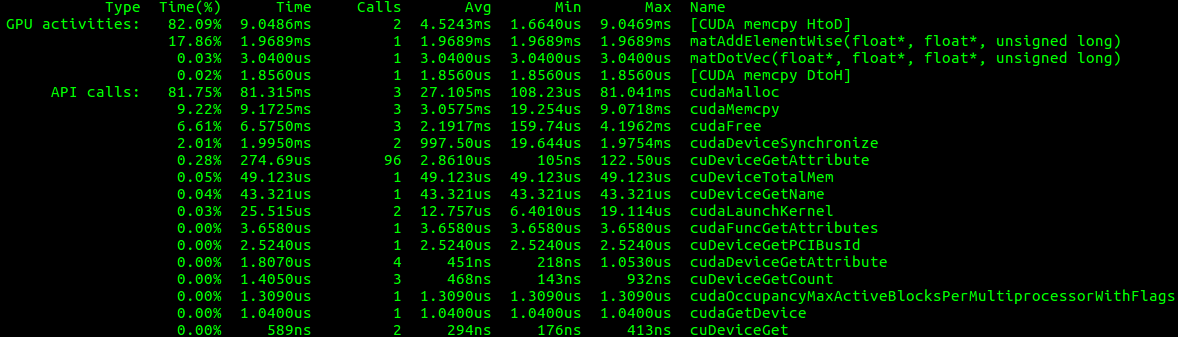
\includegraphics[width=0.95\textwidth]{fast}
    \caption{Multi Thread Matrix * Vector}
    \label{fig:fast}
\end{figure}

For the graduate portion of the assignment you can see the single-threaded 
performance via Figure \ref{fig:slowGrad}.

\begin{figure}[h]
    \centering
    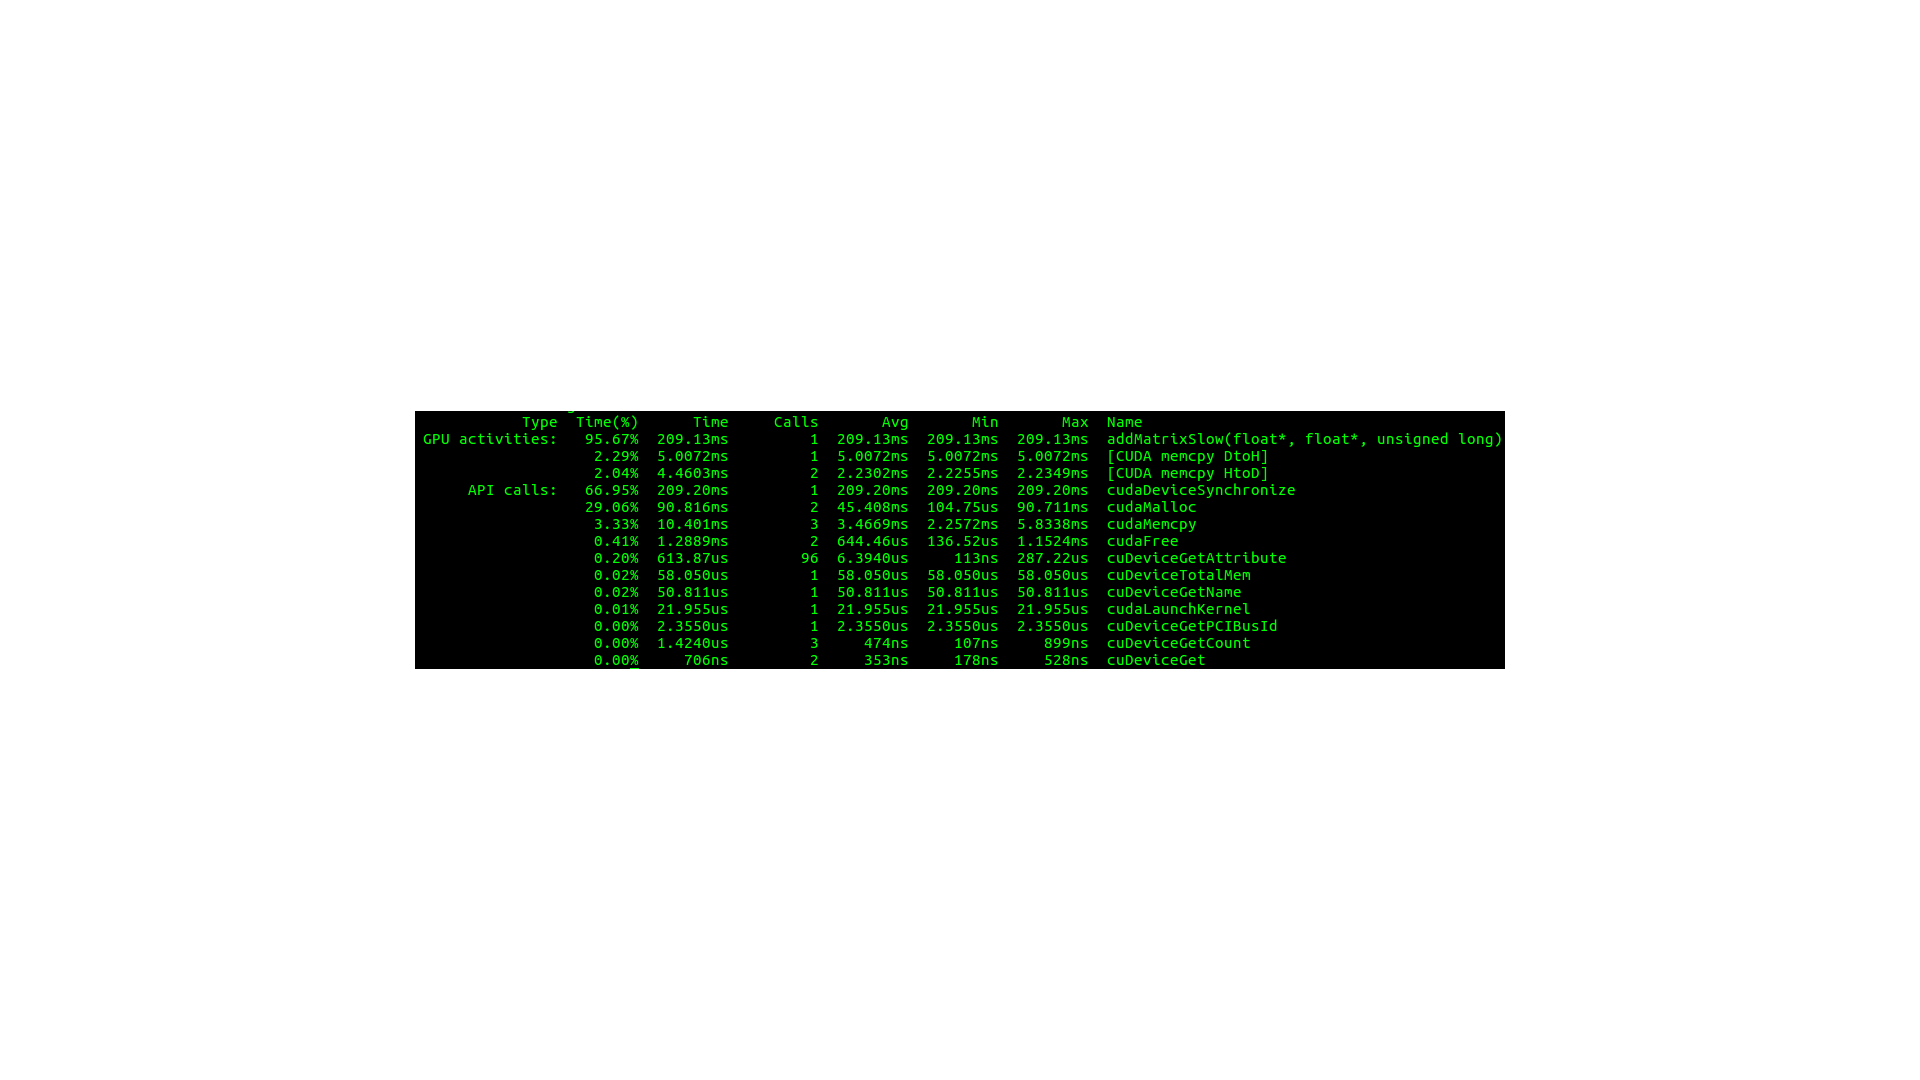
\includegraphics[width=0.95\textwidth]{slowGrad}
    \caption{Single Thread Matrix + Matrix}
    \label{fig:slowGrad}
\end{figure}

The full parallel implementation performance can be seen in Figure \ref{fig:fastGrad}.

\begin{figure}[h]
    \centering
    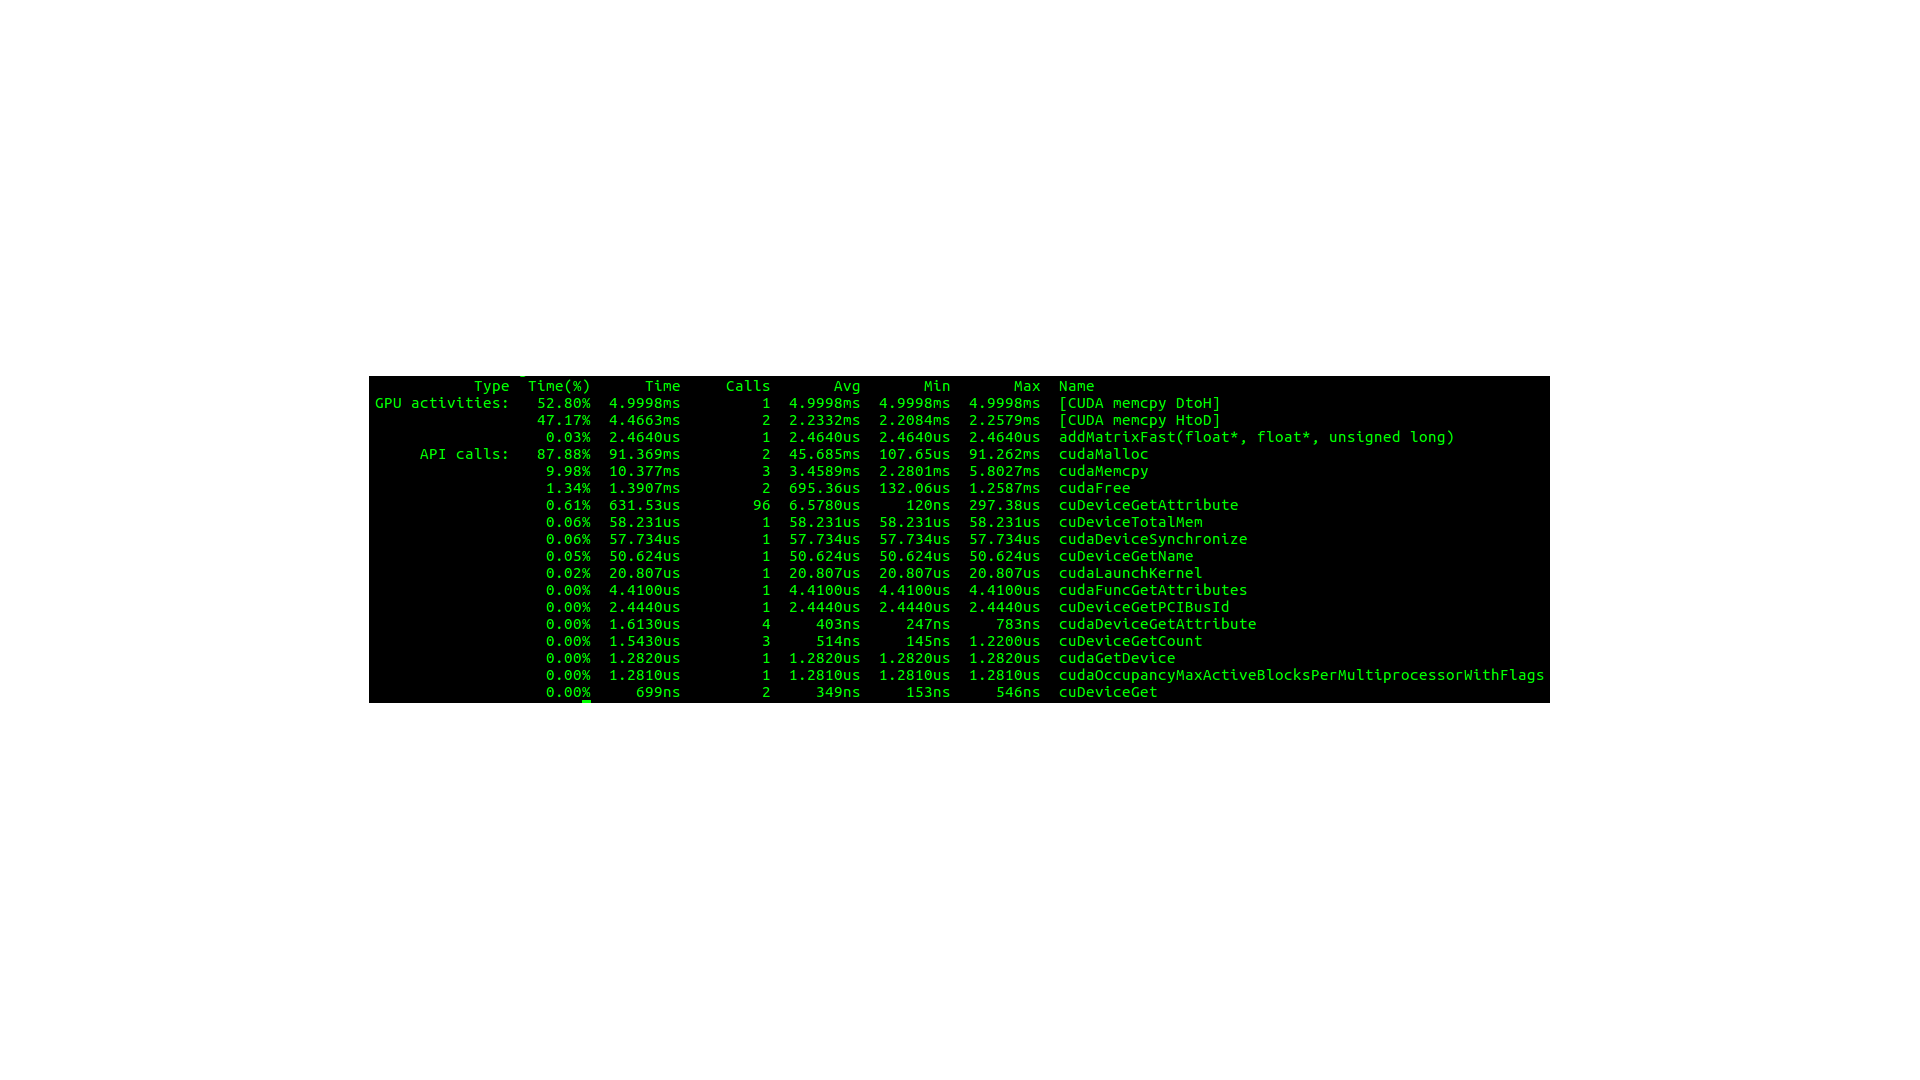
\includegraphics[width=0.95\textwidth]{fastGrad}
    \caption{Multi Thread Matrix + Matrix}
    \label{fig:fastGrad}
\end{figure}

If we compare the runtime of the single-threaded and multi-threaded functions we 
see they took $209130us$ and $2.46us$ respectively. That is a speedup of about 
$85,012$ times faster utilizing the full power of the CUDA cores. We can then 
calculate the Karp-Flatt metrix using $p=1024$ as:

$$e = \frac{\frac{1}{\psi} - \frac{1}{p}}{1 - \frac{1}{p}}$$
$$\frac{1}{\psi} = 0.000011763$$
$$\frac{1}{p} = 0.000976562$$

Which yields a Karp-Flatt metric of:
$$e = -0.000965742$$

At first I believed there was no way it could be a negative number but then I 
realized since we are not taking into account overhead it is in fact possible 
because each operation is 100\% independent of the other operations, it is 
\textbf{fully} parallelizable. If 100\% of the operations are parallelizable 
then it is possible to break this metric. Interesting.


\section{Description of what you have submitted}
Included in the submission is the code needed to compile the program, a Makefile 
to compile said code, and a detailed writeup of the assignment in pdf form.


\end{document}
